\chapter{Reflectivity Simulations}\label{multilayerdepositions}
In order to obtain structural parameters for the samples, the experimental reflectivity curves need to be fitted to mathematical simulations for each sample. There are several possible mathematical descriptions that can be used, within this work there are two different descriptions that are applied based on the software that has been used. Specular reflectivity is used described using the Paratt recursion formula, whilst the off-specular simulation is described using the Born-approximation. Both of these formalisms are described in this chapter.

\section{Parrat recursion}
The specular reflectivity of the samples is simulated using the Paratt recursion formalism. This description recursively accounts for the reflection from each subsequent interface in order to simulate the total intensity at detector. For a multilayer with a certain amount of layers, the reflectivity for the j'th layer can be calculated using: 
\begin{equation}
	\chi_j = \frac{R_j}{T_j}  = e^{-2ik_{z,j} z_j}   \frac{r_{j,j+1}+\chi_{j+1}e^{2ik_{z,j}z_j}}{1+r_{j,j+1}\chi_{j+1}+e^{2ik_{z,j}z_j}}
\end{equation}
$R_j$ and $T_j$ in this equation describe the reflected and transmitted amplitude for layer $j$. The fraction of these, $\chi_j$ therefore describes the normalised intensity from each layer. The factor $r_{j,j+1}$ is the Fresnel coefficient for the interface, and can be written as:
\begin{equation}
	r_{j,j+1} =  \frac{k_{z,j} - k_{z,j+1}}{k_{z,j} + k_{z,j+1}}
	\end{equation}
It follows from this description that this formalism is recursive, the reflectivity of layer j+1 is required to calculate the reflectivity of the j'th layer. To solve this equation, we can use $T_1$ = 1 and $R_{N+1} = 0$ as starting point, this equates to the incident wave having full transmission at $T_1$, and to no reflection from the substrate at $R_{N+1}$. This formalism is commonly used to simulate the specular reflection for neutrons and X-rays in reflectivity simulation software.
\section{Born Approximation}\label{bornapproximation}
The Born approximation (BA) was proposed as early as 1926 by Max Born. To get to this approximation, we may first start with the general time-independent Schrödinger equation:
\begin{equation}
	\qty(\frac{\hbar^2}{2m} \nabla^2 + V(\vb{r}))\Psi(\vb{r}) = E \Psi(\vb{r}) 
\end{equation}
We can re-write this as:
\begin{equation}
\qty(\nabla^2 + k^2)\Psi(\vb{r}) = \frac{2m}{\hbar}^2 V(\vb{r})\Psi(\vb{r}) 
\end{equation}
Where $k^2 = \frac{2m}{\hbar}^2$. The general solution to this equation can be expressed as an integral:
\begin{equation}
\Psi(\vb{r}) = \int G(r-r')V(\vb{r})\Psi(\vb{r})d^3r'
\end{equation}
The factor G in this equation is known as Green’s function, which can be obtained by solving the point source equation:
\begin{equation}
\qty(\nabla^2 + k^2)G(r-r') = \delta(r-r')
\end{equation}
Solving this for the Green's function gives us the integral form for the Schrödinger equation.
\begin{equation}
\label{bornscatteredwave}
\Psi(\vb{r}) = e^{i\vb{k}_0\cdot \vb{r}} - \frac{m}{2 \pi \hbar^2} \int \frac{e^{ik|r-r'|}}{\qty|r-r'|}V(r')\Psi(r')d^3 r'
\end{equation}
This equation can be solved approximately using the so-called Born series. The zero’th order solution of the Born approximation is given by a planar wave: 
\begin{equation}
		\Psi_0(\vb{r})  = e^{i\vb{k}_0\cdot \vb{r}}
\end{equation}
The first order solution is then given by inserting the solution for $\Psi_0$ into the integral of the general equation expressed in equation \ref{bornscatteredwave}. This then gives us:
\begin{eqnarray}
	\Psi_1(\vb{r}) &&= e^{i\vb{k}_0\cdot \vb{r}} - \frac{m}{2 \pi \hbar^2} \int \frac{e^{ik|r-r_1|}}{\qty|r-r_1|}V(r_1)\Psi_0(\vb{r}_1)d^3 r_1
 \\ 
	&&= e^{i\vb{k}_0\cdot \vb{r}} - \frac{m}{2 \pi \hbar^2} \int \frac{e^{ik|r-r_1|}}{\qty|r-r_1|}V(r_1)e^{i\vb{k}_0\cdot \vb{r}}d^3 r_1
\end{eqnarray}
 The second order can then be found by inserting this first order solution into equation \ref{bornscatteredwave}. By continuing this way, any order can be obtained, but for most cases only the first order approximation is actually used.
\subsection{The Distorted Wave Born Approximation}
When the scattering intensity becomes very large, the assumption of a planar wave in the conventional BA no longer holds, scattering entities themselves can introduce perturbations into the field and the wave therefore needs to be described as a distorted wave, a superposition of a downwards and upwards travelling planar wave. This is the underlying principle of the Distorted Wave Born Approximation (DWBA), which is the formalism that is used to simulate off-specular scattering in this work. The described wave function has a distorted form that can be described as downward and upward travelling waves for both the scattered and incident waves:
\begin{equation}
	\psi_w(\vb{r}) = \psi_w^-(\vb{r}) + \psi_w^+(\vb{r}), w = i, f.
\end{equation}
Where $\psi_w^-$ describes the downwards wave while $\psi_w^+$ describes the upwards wave. The relevant scattering elements can then be described using Dirac notation as follows:
\begin{equation}\label{distortedbornexpansion}
	\mel{\psi_i}{\delta v}{\psi_f} = \mel*{\psi_i^-}{\delta v}{\psi_f^+} + \mel*{\psi_i^-}{\delta v}{\psi_f^-} + \mel*{\psi_i^+}{\delta v}{\psi_f^+} + \mel*{\psi_i^+}{\delta v}{\psi_f^-}
\end{equation} 
Where $\delta v$ describes a perturbation on the scattering potential that the incident wave experiences. If we expand the left-hand side in the integral notation we get:
\begin{equation}
	\mel{\psi_i}{\delta v}{\psi_f} = \int e^{i\vb{k}_i\vb{r}}\delta v e^{i\vb{k}_f\vb{r}}d^3 r = \int \delta v e^{i\vb{q}\vb{r}}d^3 r 
\end{equation}
 Which gives us the Fourier transform of the perturbed potential $\delta v$, which is what is being measured at the detector. Note how the first term on the right-hand side in equation \ref{distortedbornexpansion} simply describes the interaction with the downwards and the upwards wave, which is the usual term as used by the conventional BA. The additional terms are added upon this in the DWBA, and these describe the additional scattering effects for intense scattering. These terms are all illustrated in figure \ref{dwba_terms}.
\begin{figure}
	\centering
	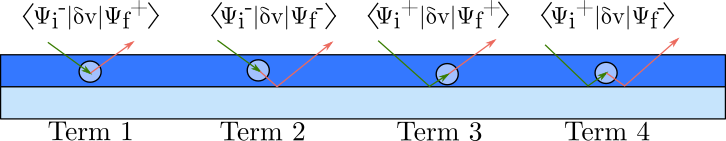
\includegraphics[width=\textwidth]{dwba_terms.png}
	\caption{While these two multilayers have roughly the same interface width, the sample on the right-hand side looks much more smooth due to the higher latteral correlation length. The latteral correlation length describes the cut-off length scale where an interface begins to look smooth.}
	\label{dwba_terms}
\end{figure}

\section{Sample description}
The samples themselves need to be described in the simulation software in order to fit the experimental data with the simulated formalism. In order to do this in a meaningful way, some approximations need to be made. It is easy to describe the sample in as much detail as possible, and let the software fit for all possible parameters, but that leaves the possibility of overfitting, losing all physical meaning behind the result. It is therefore better to make a robust and simple model, than a complicated one that is clearly overfitted. As the mathematician George Box famously said, ‘all models are wrong, but some models are useful’. Our task is not to find a model that gives a perfect fit to our data, it is our task instead to find a model that actually is useful.  In our case this means a model that reliably gives physically correct information about the structural parameters of the sample.
The samples in this work are all described with such as description. A stack of an N amount of bilayers consisting of Ni and Ti are deposited on top op a Si substrate. A thin layer of SiO2 is assumed between the Si substrate and the multiplayer stack. On top of the multilayer stack, an oxide layer is assumed to exist as well. A sketch describing this can be seen in figure \ref{modeldescription}.

\begin{figure}[h]
	\centering
	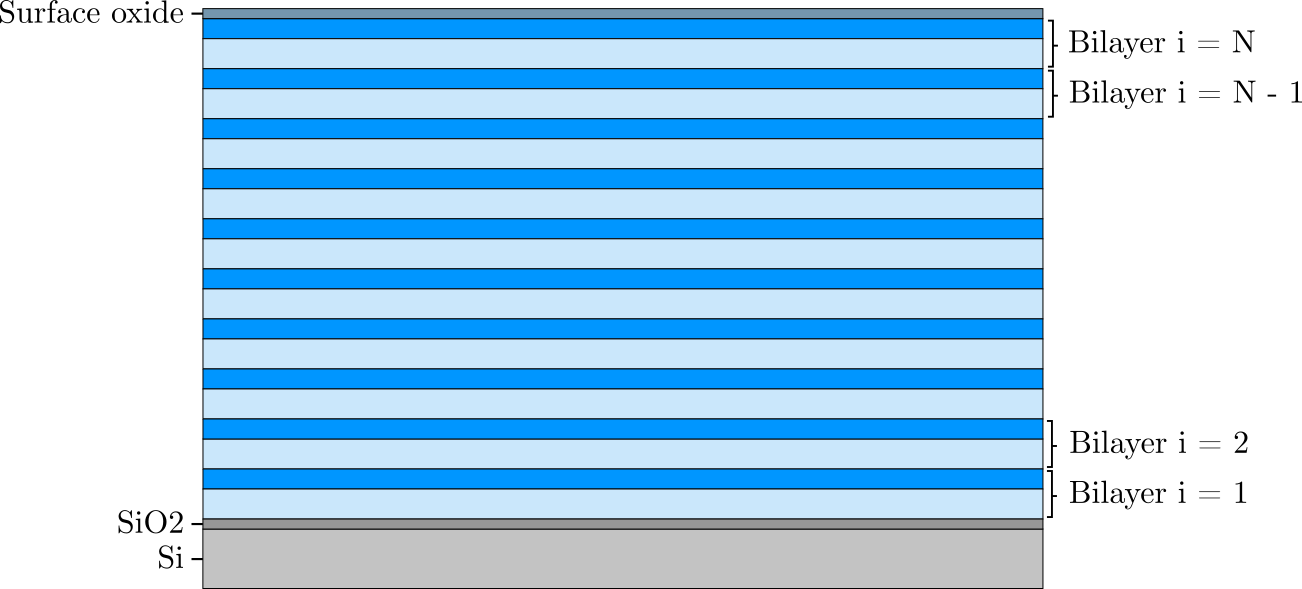
\includegraphics[width=\textwidth]{multilayer_model.png}
	\caption{While these two multilayers have roughly the same interface width, the sample on the right-hand side looks much more smooth due to the higher latteral correlation length. The latteral correlation length describes the cut-off length scale where an interface begins to look smooth.}
	\label{modeldescription}
\end{figure}

While the initial interface width of the Ni and Ti layers are considered independent from each other, the accumulation of the interface width is assumed to be equal. The total interface width for a Ni and Ti layer in the stack, is therefore determined by:
\begin{eqnarray}
	\sigma_{\textrm{Ti}} = A \cdot i + \sigma_{\textrm{Ti,i}} \\
	\sigma_{\textrm{Ni}} = A \cdot i + \sigma_{\textrm{Ni,i}}
\end{eqnarray}
Where A is the accumulated interface width per bilayer, i indicates the position of the bilayer, and $\sigma_{\textrm{Ni}}$ and $\sigma_{\textrm{Ti}}$ describe the initial interface width of Ni and Ti respectively.